\documentclass[conference]{IEEEtran}
\IEEEoverridecommandlockouts
% The preceding line is only needed to identify funding in the first footnote. If that is unneeded, please comment it out.
%----------------------------------------------------------
\usepackage{cite}
\usepackage[pdftex]{graphicx}
% declare the path(s) where your graphic files are
\graphicspath{images/}
\DeclareGraphicsExtensions{.pdf,.jpeg,.png,.jpg}
\usepackage{amsmath,amssymb,amsfonts}
\usepackage{algorithmic}
\usepackage{graphicx}
\usepackage{textcomp}
\usepackage{array}
%\usepackage[caption=false,font=normalsize,labelfont=sf,textfon =sf]{subfig}
\usepackage{dblfloatfix}
\usepackage{url}
\usepackage{lipsum}
\usepackage{listings}
\usepackage{xcolor}
\def\BibTeX{{\rm B\kern-.05em{\sc i\kern-.025em b}\kern-.08em
    T\kern-.1667em\lower.7ex\hbox{E}\kern-.125emX}}
%----------------------------------------------------------
    \lstset{
        escapeinside={/*@}{@*/},
        language=Python,	
        basicstyle=\fontsize{8.5}{12}\selectfont,
        numbers=left,
        numbersep=2pt,    
        xleftmargin=2pt,
        frame=tb,
        columns=fullflexible,
        showstringspaces=false,
        tabsize=4,
        keepspaces=true,
        showtabs=false,
        showspaces=false,
        morekeywords={inline,public,class,private,protected,struct},
        captionpos=b,
        lineskip=-0.4em,
        aboveskip=10pt,
        extendedchars=true,
        breaklines=true,
        prebreak = \raisebox{0ex}[0ex][0ex]{\ensuremath{\hookleftarrow}},
        keywordstyle=\color[rgb]{0,0,1},
        commentstyle=\color[rgb]{0.133,0.545,0.133},
        stringstyle=\color[rgb]{0.627,0.126,0.941},
    }
%----------------------------------------------------------

\begin{document}

\title{Controle de braços robóticos auxiliados por visão computacional.
% \\
% {\footnotesize \textsuperscript{*} Sistemas Embarcados: Prof. Marco Reis - marco.reis@ba.docente.senai.brr}
% \thanks{Identify applicable funding agency here. If none, delete this.}
}

% \author{\IEEEauthorblockN{Marco Reis, 41650-010\IEEEauthorrefmark{1}}
% \IEEEauthorblockA{\IEEEauthorrefmark{1}Robotics & Autonomous Systems Center,
% Senai Cimatec, Salvador, Brazil}% <-this % stops an unwanted space


\author{\IEEEauthorblockN{Marco Reis}
\IEEEauthorblockA{\textit{SENAI CIMATEC} \\
% \textit{name of organization (of Aff.)}\\
Salvador, Brasil \\
marco.reis@aln.senaicimatec.edu.br}
\and
\IEEEauthorblockN{Icaro Borges de Macedo (orientador)}
\IEEEauthorblockA{\textit{SENAI CIMATEC} \\
% \textit{name of organization (of Aff.)}\\
Salvador, Brasil \\
icaro.macedo@fieb.org.br}
\and
\IEEEauthorblockN{Tiago Barretto Sant’Anna}
\IEEEauthorblockA{\textit{SENAI CIMATEC} \\
% \textit{name of organization (of Aff.)}\\
Salvador, Brasil\\
tiago.sant'anna@ba.estudante.senai.br}
\and
\IEEEauthorblockN{Samuel Luiz Silva Santana }
\IEEEauthorblockA{\textit{SENAI CIMATEC} \\
% \textit{name of organization (of Aff.)}\\
Salvador, Brasil \\
samuel.santana@ba.estudante.senai.br}
\and
% \IEEEauthorblockN{5\textsuperscript{th} Given Name Surname}
% \IEEEauthorblockA{\textit{dept. name of organization (of Aff.)} \\
% % \textit{name of organization (of Aff.)}\\
% City, Country \\
% email address or ORCID}
% \and
% \IEEEauthorblockN{6\textsuperscript{th} Given Name Surname}
% \IEEEauthorblockA{\textit{dept. name of organization (of Aff.)} \\
% \textit{name of organization (of Aff.)}\\
% City, Country \\
% email address or ORCID}
}

\maketitle

\begin{abstract}
O objetivo deste artigo é expor os problemas na automação dentro da área da robótica industrial e trabalhar para consertar esse fato. Portanto visando tornar a tecnologia robótica mais autônoma, mais especificamente os braços robóticos, desenvolvemos esse artigo que visa interromper a dependência de uma programação que limita esses robôs a fazer apenas movimentos repetitivos com peças específicas sem nenhuma capacidade de realizar outros movimentos além daqueles pré-programados. Sabemos que esse é um problema que depende de um grande acúmulo de conhecimento antes de poder ser solucionado, devido a esse fato decidimos realizar pesquisas sobre o assunto e desenvolver resultados utilizando a visão computacional. Esses resultados devem impactar diretamente no dia-a-dia da indústria, pois irá reduzir a necessidade de programar novamente um robô para cada mudança em sua função.
\end{abstract}

\begin{IEEEkeywords}
robótica, mecatrônica, manipuladores, visão computacional.
\end{IEEEkeywords}

\section{Introduction}

A robótica é uma área em crescimento no mundo, podendo se expandir até 10 vezes mais na última década \cite{Roboticonline}. Esse aumento se dá principalmente na indústria, onde o uso da robótica gera um maior aumento da produtividade \cite{robotica1}. Desse modo, é uma área que necessita de constantes avanços tecnológicos para suprir essa demanda. Porém, um problema encontrado na robótica industrial é que sua automação não consegue ser independente o suficiente. Quando se programa um braço robótico ele pode fazer o mesmo movimento diversas vezes de forma autônoma, entretanto caso a peça a ser manipulada seja deslocada, o braço não tem capacidade, de forma autônoma, de alterar sua trajetória para poder trabalhar com ela. Assim, como fazer com que um braço robótico possa pegar objetos específicos, independente de suas posições no espaço? Dessa maneira, o objetivo desse artigo é estudar e criar um algoritmo para braço robótico cuja função é coletar objetos usando visão computacional, independente de qual posição eles estejam, fazendo o uso de visão computacional. Os objetivos específicos desse artigo, são o estudo e geração do reconhecimento de peças com visão computacional, a cinemática do manipulador, a programação do manipulador e a integração da câmera com o braço robótico.  A importância desse procedimento tem como consequência uma diminuição na necessidade de reprogramação desses braços robóticos, irá facilitar a programação para poder realizar tarefas ainda mais complexas, fornecendo assim economia e efetividade. Dessa forma será realizada uma pesquisa bibliográfica, acerca de braços robóticos, visão computacional e cinemática. Esse trabalho é uma pesquisa aplicada, com objetivo exploratório, por uma abordagem qualitativa.

\section{Fundamentação teórica}

\subsection{Identificação de objetos}

Para poder fazer a identificação dos objetos foram escolhidos fazer o uso de marcos fiduciais. Esses marcos fiduciais são imagens ou objetos usados como pontos de referência para os robôs realizarem certas ações \cite{Fiducial26:online}. % Change this reference later, not use wikipedia.
Com o uso desses marcadores, facilitará na hora de identificar a posição dos objeto no espaço e sua orientação.


\begin{figure}[h!]
\centering
    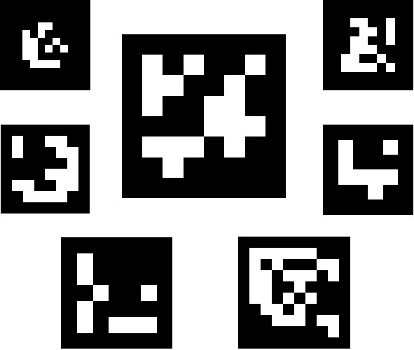
\includegraphics[width=4cm]{images/markers.jpg}
\caption{Exemplos de tags \cite{OpenCVDe76:online}}
\label{fig:tags}
\end{figure}

A figura \ref{fig:tags} mostra um exemplo dessas tags. Elas possuem padrões que são facilmente identificados pelas câmeras e se dado as suas dimensões pode se usar algoritmos para descobrir suas coordenadas no espaço. Dessa forma foi pensado em colocar uma câmera em uma posição estratégica do braço para dar uma melhor visão dos objetos e poder reconhece-los, além de usar sua posição para definir a cinemática do braço.

\begin{figure}[h!]
    \centering
        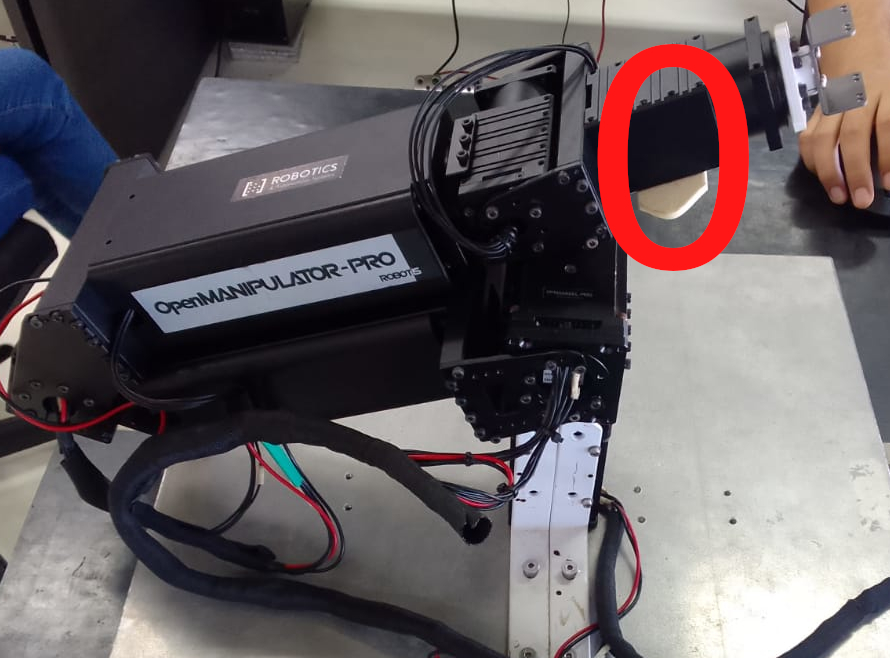
\includegraphics[width=8cm]{images/arm_marked.jpeg}
    \caption{Imagem do braço robótico}
    \label{fig:cam_arm}
\end{figure}

Por questão de praticidade foi decidido usar uma webcam para captar as imagens do ambiente, essa câmera sera colocada na parte sinalizada no braço robótico, explicitado na figura \ref{fig:cam_arm}. Assim será processado para onde a ferramenta esta direcionada.

\subsubsection{Calibração da camera}

A calibração é uma parte fundamental para conseguir parâmetros fundamentais de uma camera, com esses dados se consegue determinar onde esta um ponto 3D no espaço \cite{ArUco}. Isso é feito para obter valores, como o de pixels da camera, coeficientes de distorção e centro óptico do sensor\cite{ArUco}.

\begin{figure}[h!]
    \centering
        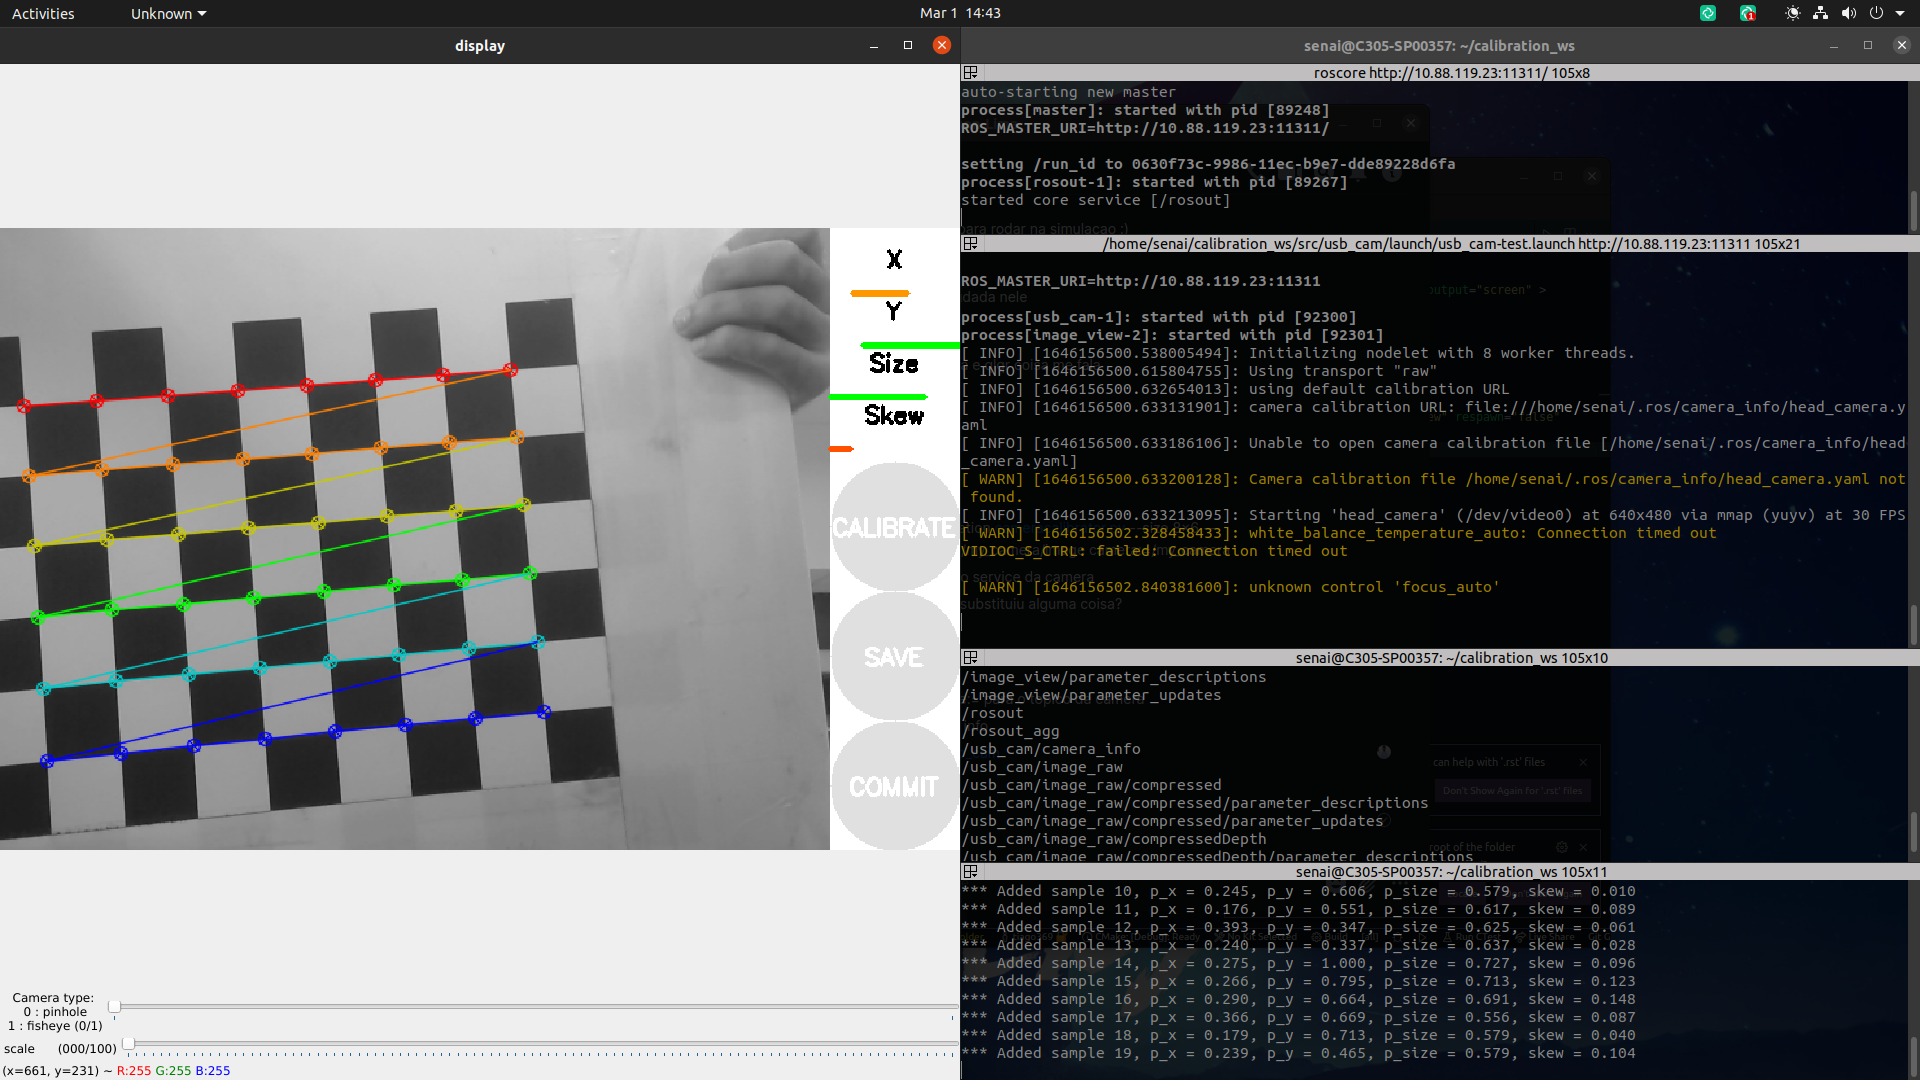
\includegraphics[width=9cm]{images/calibration.png}
    \caption{Calibração}
    \label{fig:calibration}
\end{figure}

Dessa forma a calibração foi feita usando o \textit{ROS Noetic}, com um pacote especifico para calibração\cite{camera_calibration:online} e um pacote próprio para conectar a webcam no pc\cite{usbcamRO60:online}. Parte do processo da calibração pode ser mostrado na imagem\ref{fig:calibration}. Com esse processo foi gerado um arquivo comprimido com todas as informações necessárias para configurar a câmera. Assim foi finalizado essa etapa do processo

\subsection{Braço robótico}

O braço escolhido foi um braço robótico do tipo universal\cite{robotica1}, também chamado de antropomórfico. Esse tipo de braço foi escolhido devido a grande quantidade de usos que ele possui\cite{robotica1}.

\begin{figure}[h!]
    \centering
        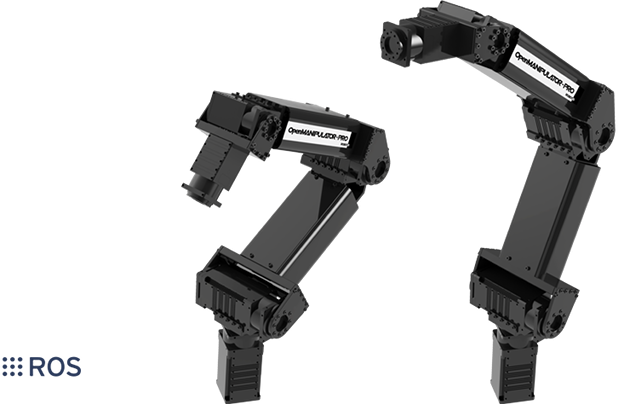
\includegraphics[width=9cm]{images/product_img.png}
    \caption{Open Manipulator\cite{OpenMANI65:online}}
    \label{fig:open_m}
\end{figure}

Dessa forma foi escolhido o manipulador \textit{Open Manipulator}. Mostrado na imagem\ref{fig:open_m}. Assim o braço conseguira realizar movimentos complexos.

Outra vantagem de utilizar esse braço é que possui uma integração com o ROS, permitindo o uso de diversos pacotes que facilitam a programação.

\subsection{Integração braço robótico com camera}

Para poder coletar os objetos o manipulador precisa considera a posição do objeto em relação a camera e a posição da camera em relação ao manipulador. Para poder realizar isso é utilizado um conjunto de cálculos matemático conhecido como transformação de coordenadas.

Ja existem bibliotecas prontas que realizam esse trabalho matemático\cite{tfROSWik45:online}. Ja que é necessário conseguir identificar onde a ferramenta e a camera se encontram em no espaço.



%----------------------------------------------------------
\bibliographystyle{IEEEtran}
\bibliography{Bibliography}
%CRITICAL: do not change the above two lines!!!
%----------------------------------------------------------

% \vspace{12pt}
% \color{red}
% Course templates contain guidance text for composing and formatting Course papers. Please ensure that all template text is removed from your course paper prior to submission to the lecturer. Failure to remove the template text from your paper may result in your paper not being accepted.

\end{document}
